\documentclass[aspectratio=169,11pt,hyperref={colorlinks=true}]{beamer}
\usetheme{boxes}
\setbeamertemplate{navigation symbols}{}
\definecolor{openstack}{RGB}{149,0,4}
\setbeamercolor{titlelike}{fg=openstack}
\setbeamercolor{structure}{fg=openstack}
\hypersetup{colorlinks,urlcolor=openstack}
\setbeamertemplate{footline}[frame number]
% Inserting graphics
\usepackage{graphicx}
% Side-by-side figures, etc
\usepackage{subfigure}
% Code snippits
\usepackage{listings}
% Color stuff
\usepackage{color}
\usepackage{amsmath}
\usepackage{tikz}
\newcommand\RBox[1]{%
  \tikz\node[draw,rounded corners,align=center,] {#1};%
}
\usepackage{hyperref}
%\usecolortheme{buzz}
%\usecolortheme{wolverine}
%\usetheme{Boadilla}
\usepackage[T1]{fontenc}

\definecolor{mygreen}{rgb}{0,0.6,0}
\definecolor{mygray}{rgb}{0.5,0.5,0.5}
\definecolor{mymauve}{rgb}{0.58,0,0.82}

\lstset{%
  backgroundcolor=\color{white},   % choose the background color; you must add \usepackage{color} or \usepackage{xcolor}
  breakatwhitespace=false,         % sets if automatic breaks should only happen at whitespace
  breaklines=true,                 % sets automatic line breaking
  captionpos=b,                    % sets the caption-position to bottom
  commentstyle=\color{openstack},  % comment style
  extendedchars=true,              % lets you use non-ASCII characters; for 8-bits encodings only, does not work with UTF-8
  keepspaces=true,                 % keeps spaces in text, useful for keeping indentation of code (possibly needs columns=flexible)
  keywordstyle=\color{blue},       % keyword style
%  otherkeywords={*,...},           % if you want to add more keywords to the set
  numbersep=5pt,                   % how far the line-numbers are from the code
  numberstyle=\tiny\color{mygray}, % the style that is used for the line-numbers
  rulecolor=\color{black},         % if not set, the frame-color may be changed on line-breaks within not-black text (e.g. comments (green here))
  showspaces=false,                % show spaces everywhere adding particular underscores; it overrides 'showstringspaces'
  showstringspaces=false,          % underline spaces within strings only
  showtabs=false,                  % show tabs within strings adding particular underscores
  stringstyle=\color{openstack},   % string literal style
}

\setbeamerfont{caption}{series=\normalfont,size=\fontsize{6}{8}}
\setbeamertemplate{caption}{\raggedright\insertcaption\par}

\setlength{\abovecaptionskip}{0pt}
\setlength{\floatsep}{0pt}

\author[Matthew Treinish & Jeremy Stanley]{%
    \texorpdfstring{%
        \begin{columns}
            \column{.45\linewidth}
            \centering
            Matthew Treinish\\
            \href{mailto:mtreinish@kortar.org}{mtreinish@kortar.org}\\
        \texttt{mtreinish on Freenode}
        \column{.45\linewidth}
            \centering
            Jeremy Stanley\\
            \href{mailto:fungi@yuggoth.org}{fungi@yuggoth.org}\\
            \texttt{fungi on Freenode}
        \end{columns}
        }
    {Matthew Treinish & Jeremy Stanley}
}
\date{May 11, 2017}

\title[Firehose: a Unified Message Bus for Infra Services
\hspace{2em}\insertframenumber/\inserttotalframenumber]{Firehose: a Unified Message Bus for Infra Services}

\begin{document}

{%
\setbeamertemplate{background canvas}{
\includegraphics[width=\paperwidth,height=\paperheight]{background_title.png}}
\setbeamertemplate{footline}{}
\begin{frame}[noframenumbering]
    \setbeamercolor{titlelike}{fg=white}
    \setbeamercolor{structure}{fg=white}
    \setbeamercolor{normal text}{fg=white}
    \hypersetup{colorlinks,urlcolor=white}
    \setbeamercolor{author}{fg=white}
    \setbeamercolor{date}{fg=white}
    \setbeamercolor{background}{bg=openstack}
    \titlepage{}
    \centering
    \href{https://github.com/mtreinish/firehose/tree/boston-summit}{https://github.com/mtreinish/firehose/tree/boston-summit}
\end{frame}
}

\section{OpenStack Infrastructure}
\begin{frame}
\frametitle{OpenStack Infrastructure}
\centering
\textbf{Imagine a big, complicated diagram here.}
\end{frame}

\subsection{Firehose Introduction}
\begin{frame}
	\frametitle{Firehose}
    \begin{itemize}
        \item An MQTT broker for the OpenStack community infrastructure
        \item Has anonymous, read-only access via MQTT on 1883/tcp
        \item SSL/TLS MQTT also available on 8883/tcp
        \item Websockets supported (but temporarily disabled)
    \end{itemize}
\end{frame}

\section{MQTT}
\begin{frame}
	\frametitle{MQTT}
    \begin{itemize}
        \item Pub/sub messaging protocol
        \item Formerly MQ Telemetry Transport
        \item ISO/IEC PRF 20922
        \item Protocol dates back to 1999
        \item Lightweight design, low bandwidth
    \end{itemize}
\end{frame}

\begin{frame}
    \frametitle{MQTT Topics}
    \begin{itemize}
        \item Topcis are heirarchical
        \item Support wild carding
    \end{itemize}
\end{frame}

\begin{frame}
    \frametitle{MQTT Brokers}
\end{frame}

\begin{frame}
    \frametitle{MQTT Clients}

\end{frame}


\section{Firehose in detail}
\begin{frame}
    \frametitle{The Firehose}

\end{frame}

\begin{frame}
    \frametitle{Mosquitto}
    \begin{columns}[T]
        \begin{column}{.48\textwidth}
            \begin{itemize}
                \item MQTT broker implemented in C
            \end{itemize}
        \end{column}
        \begin{column}{.48\textwidth}
            
\includegraphics[width=\textwidth]{mosquitto.png}
        \end{column}
    \end{columns}
\end{frame}

\subsection{Services in the Firehose}
\begin{frame}
    \frametitle{Services Using the Firehose}
    \begin{center}
        \begin{tabular}{ccc}
            \hline
            \textbf{Service} & \textbf{Base Topic} & \textbf{Source of Messages}\\
            \hline
            Ansible & ansible & \href{http://git.openstack.org/cgit/openstack-infra/system-config/tree/modules/openstack_project/files/puppetmaster/mqtt.py}{Ansible MQTT Callback Plugin} \\
            Gerrit & gerrit & \href{http://git.openstack.org/cgit/openstack-infra/germqtt/}{germqtt} \\
            Launchpad & launchpad & \href{http://git.openstack.org/cgit/openstack-infra/lpmqtt/}{lpmqtt} \\
            Subunit Gearman Worker & gearman-subunit & \href{http://git.openstack.org/cgit/openstack-infra/puppet-subunit2sql/tree/files/subunit-gearman-worker.py}{subunit-gearman-worker} \\
        \end{tabular}
    \end{center}
\end{frame}

\begin{frame}
    \frametitle{Typical Firehose Load}
    \centering
    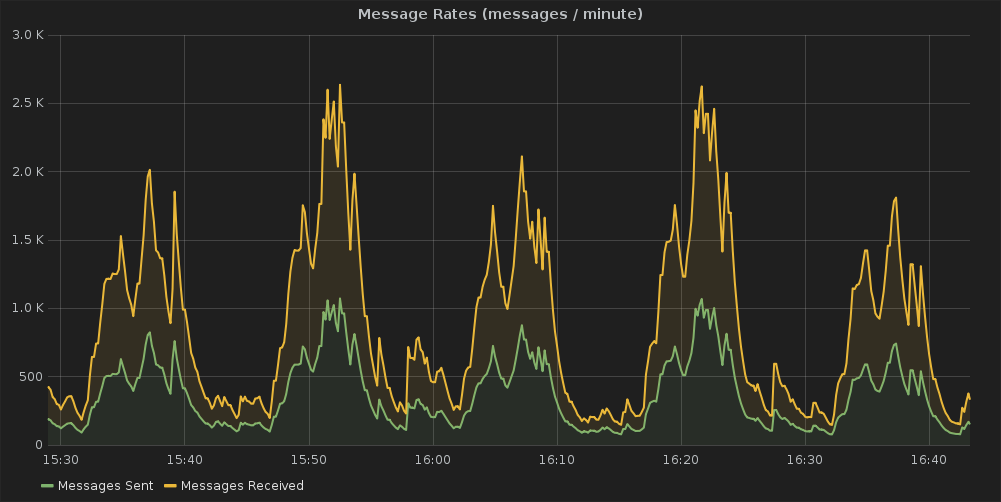
\includegraphics[width=.9\textwidth]{typical_message_rates.png}
\end{frame}

\begin{frame}
    \centering
    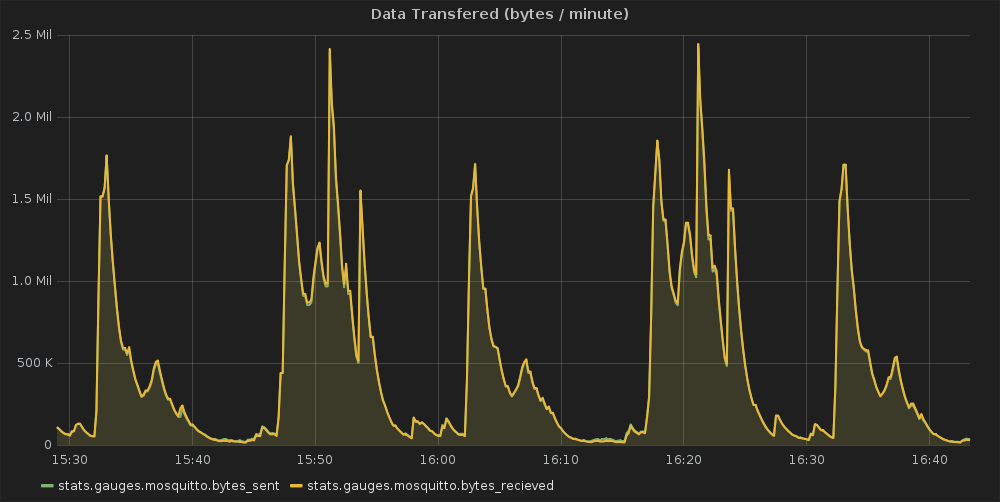
\includegraphics[width=.9\textwidth]{typical_data_rates.png}
\end{frame}

\begin{frame}
    \frametitle{The limits of scaling}
    \centering
    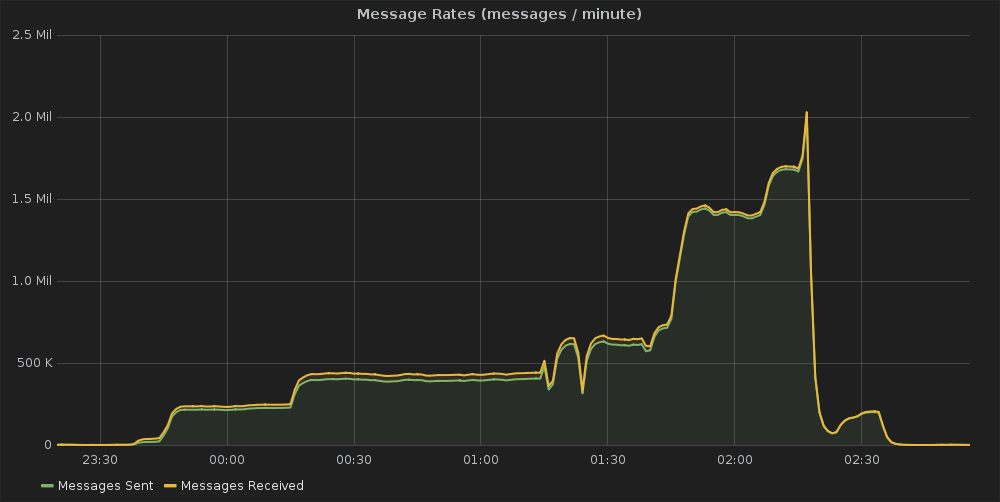
\includegraphics[width=.9\textwidth]{manual-load-test.png}
\end{frame}

\begin{frame}
    \begin{columns}[T]
        \begin{column}{.48\textwidth}
            \textbf{CPU Usage:}\\
            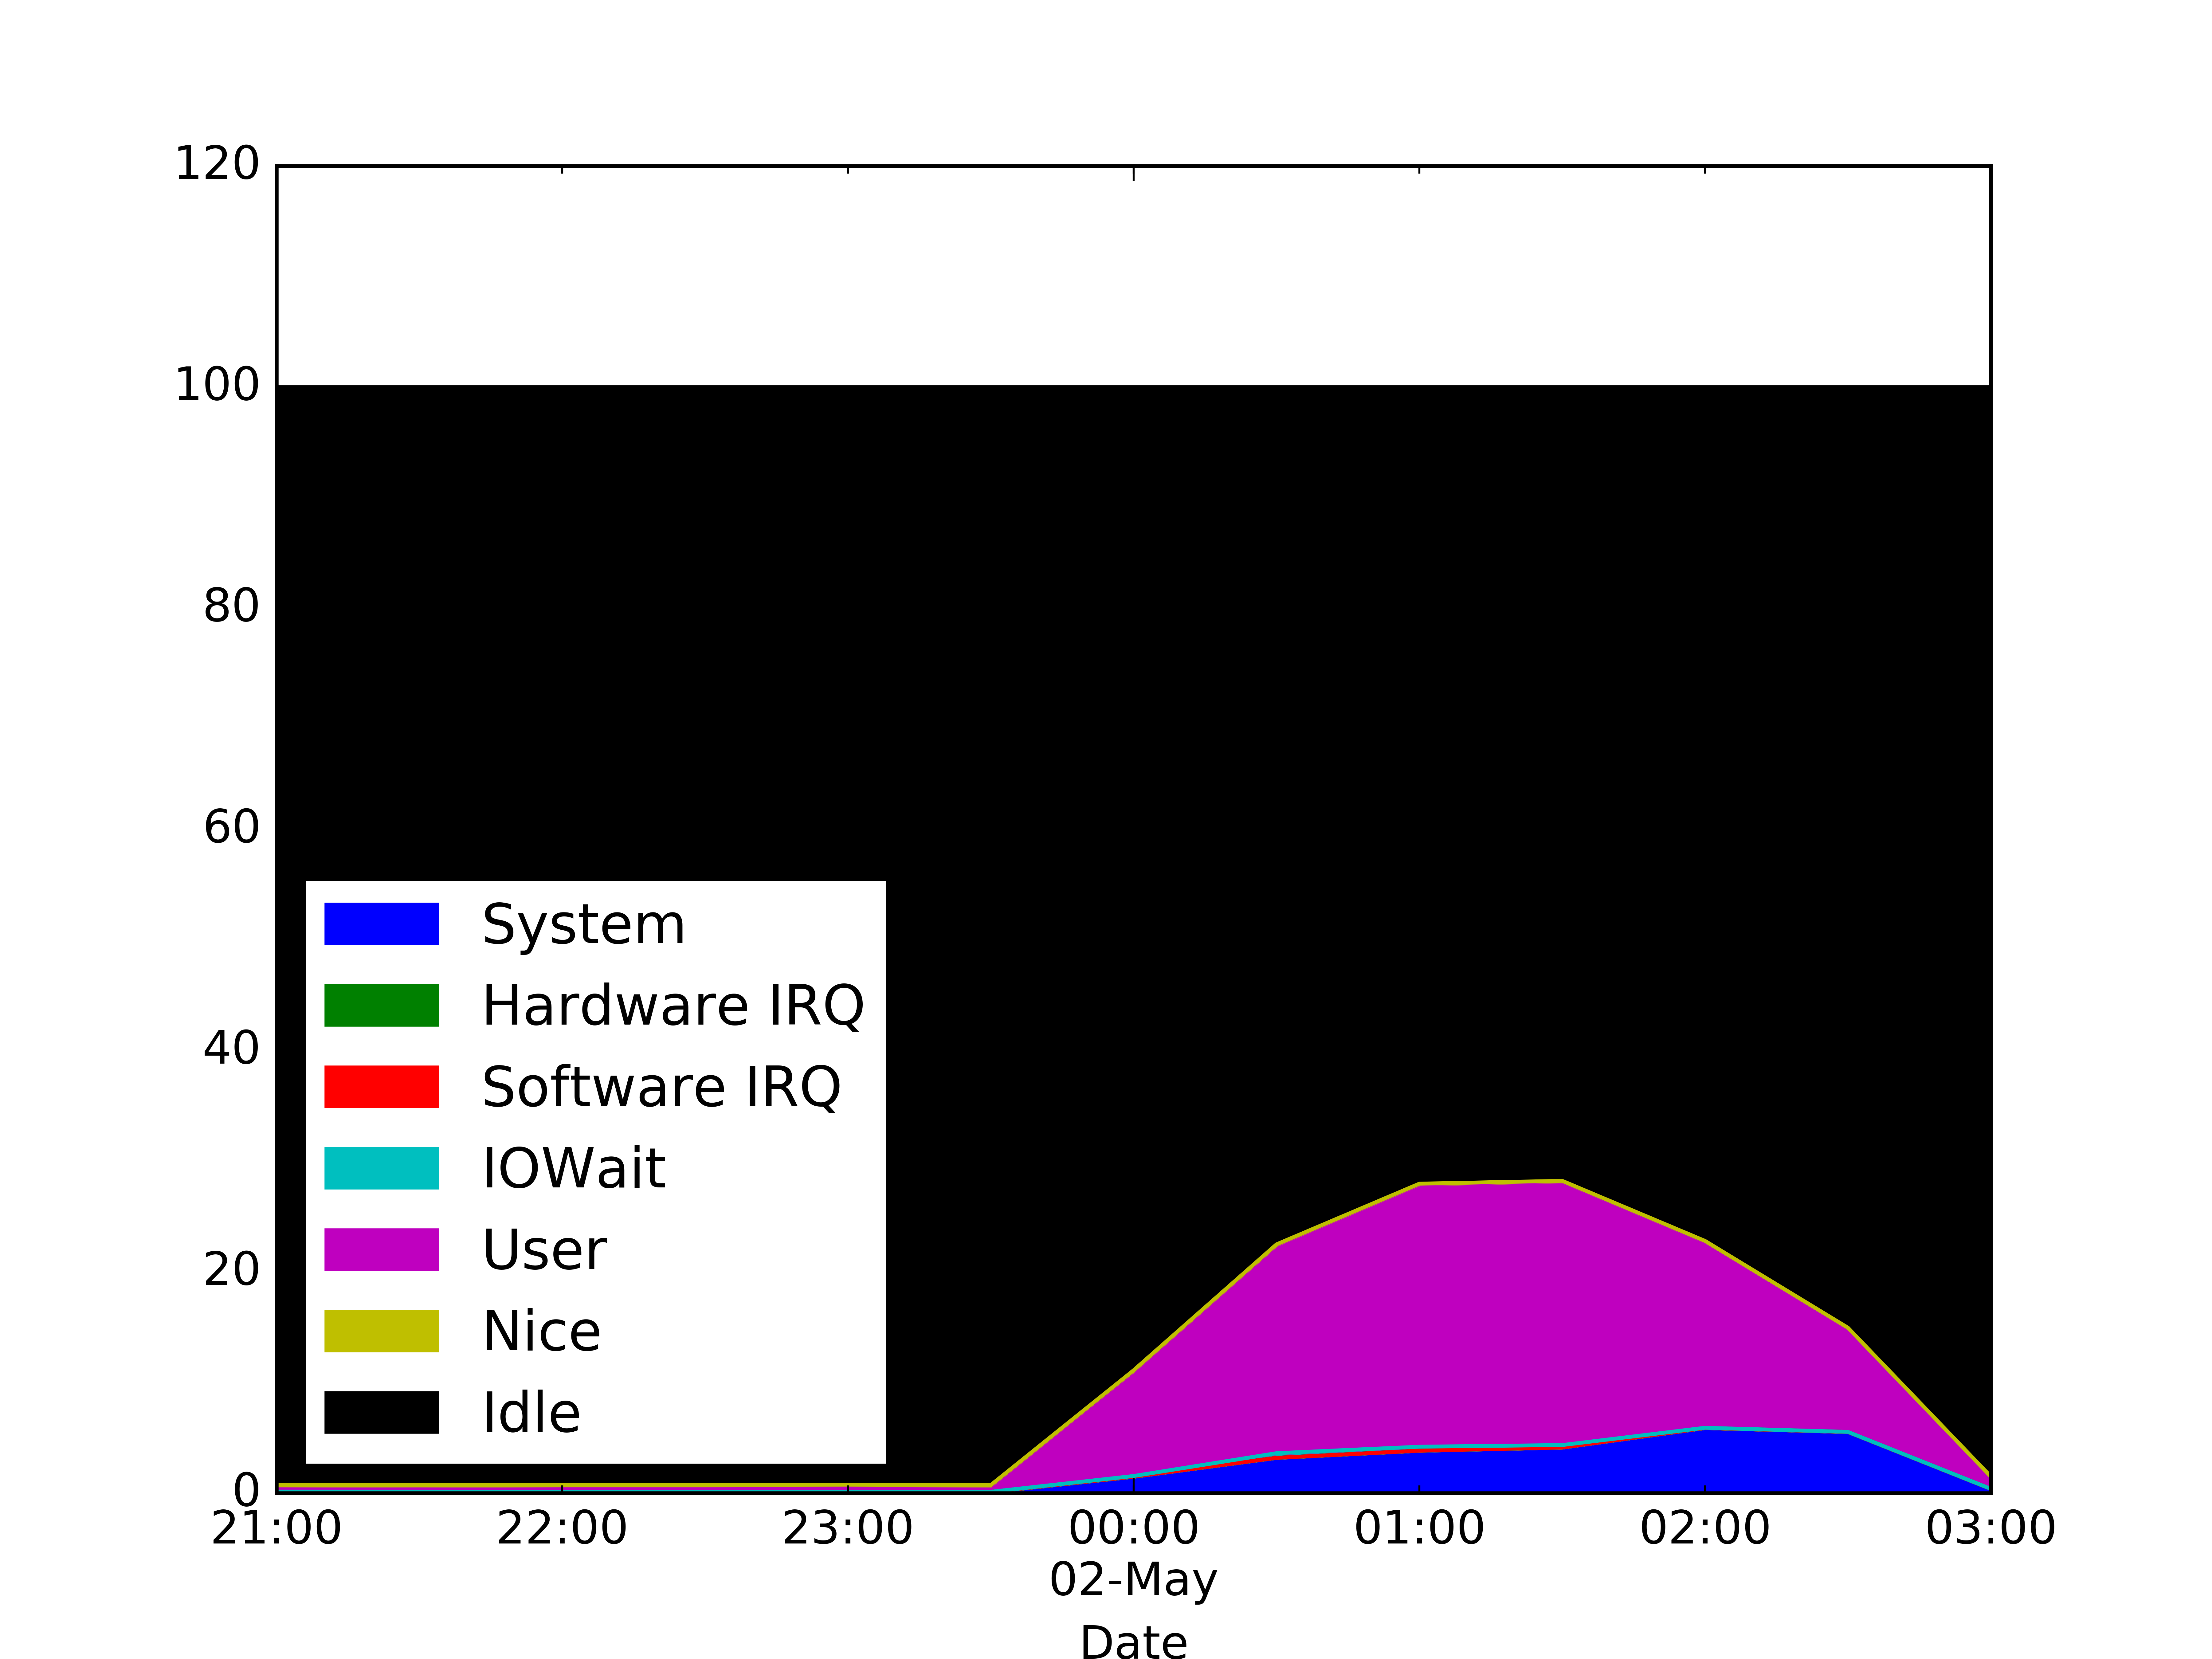
\includegraphics[width=\textwidth]{manual_load_cpu_usage.png}
        \end{column}
        \begin{column}{.48\textwidth}
            \textbf{Memory Usage:}\\
            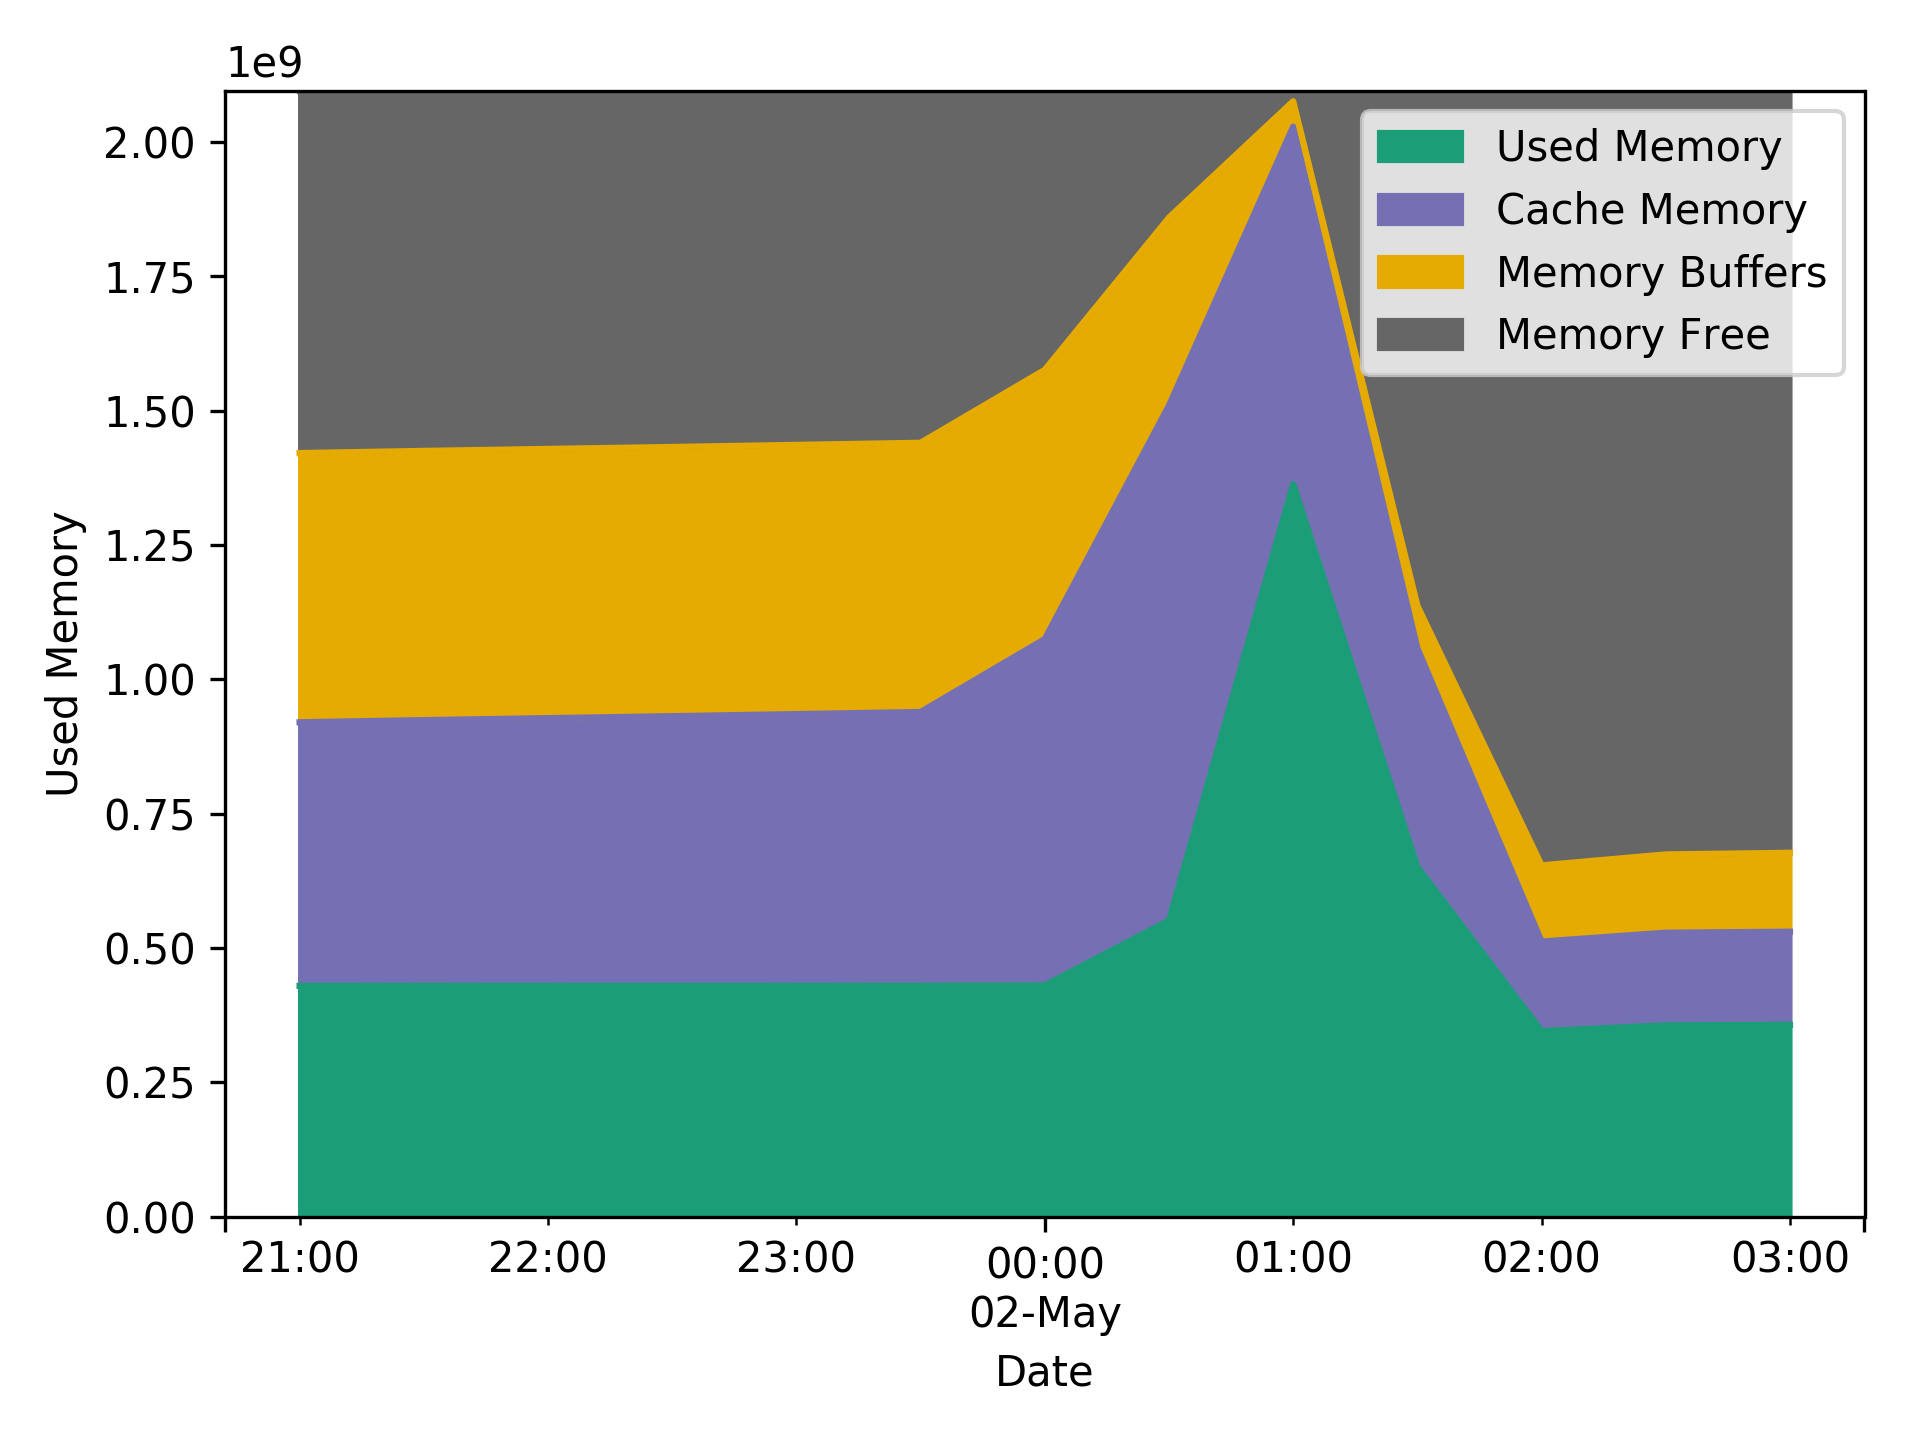
\includegraphics[width=\textwidth]{manual_load_ram_usage.png}
        \end{column}
    \end{columns}
\end{frame}

\begin{frame}
    \frametitle{Using Firehose}
    Example mosquitto client subscriber command line (provided in a
mosquitto-clients package on many distros):

    \begin{center}
        \texttt{mosquitto\_sub \--h firehose.openstack.org \--\--topic '\#'}
    \end{center}
\end{frame}

\begin{frame}
    \frametitle{Listen for all Nova Comments in python}
    \begin{itemize}
        \item \textbf{CLI:}\\
            \textit{mosquitto\_sub \--h firehose.openstack.org \--\--topic gerrit/openstack/nova/comment-added}
        \item \textbf{Python:}\\
            \lstinputlisting[basicstyle=\tiny,language=python]{python_nova_sub.py}
    \end{itemize}
\end{frame}

% Add anotuer example

\begin{frame}
    \frametitle{Potential Applications for Firehose}
\end{frame}

\section{Future Plans}
\begin{frame}
    \frametitle{Future Plans}
    \begin{itemize}
        \item Add germqtt subscription support to:
            \begin{itemize}
                \item Zuul v3+
            \end{itemize}
        \item Add more publishers:
            \begin{itemize}
                \item Nodepool daemons
                \item Zuul v3+
                \item (your favorite service here)
            \end{itemize}
    \end{itemize}
\end{frame}

\section{More Information}
\begin{frame}
\frametitle{Where to get more information}
    \begin{itemize}
        \item openstack-infra ML\: \href{mailto:openstack-infra@lists.openstack.org}{openstack-infra@lists.openstack.org}
        \item \#openstack-infra on Freenode
	\item \href{http://docs.openstack.org/infra/system-config/firehose.html}{http://docs.openstack.org/infra/system-config/firehose.html}
    \item \href{https://docs.openstack.org/infra/system-config/firehose_schema.html}{https://docs.openstack.org/infra/system-config/firehose\_schema.html}
	\item \href{http://specs.openstack.org/openstack-infra/infra-specs/specs/firehose.html}{http://specs.openstack.org/openstack-infra/infra-specs/specs/firehose.html}
	\item \href{http://mqtt.org/}{http://mqtt.org/}
	\item \href{https://mosquitto.org/}{https://mosquitto.org/}
    \end{itemize}
\end{frame}

\end{document}
